\documentclass{SCreport}
\usepackage[utf8]{inputenc}
\usepackage[T1]{fontenc}
\usepackage{float}
\setcounter{tocdepth}{2}
\reporttype{SC20}
\reportauthor{A.~Magnusson\footnote{\spc} and N.~Davies\footnote{TeTakina Ltd}}
\reporttitle{Scoping the Next Generation of Tuna Stock Assessment
  Software:\\Progress Report and Outline of Options (Project 123)}
\reportnumber{\tpnum/SA-WP-01}
\reportdate{14 August 2024}
\hyphenation{computational consideration desired assessment future replacement
  development simple progression synthesis}
\begin{document}

\wcpfctitlepage

\tableofcontents
\newpage

\section{Executive summary}

\begin{figure}[H]
  \centering
  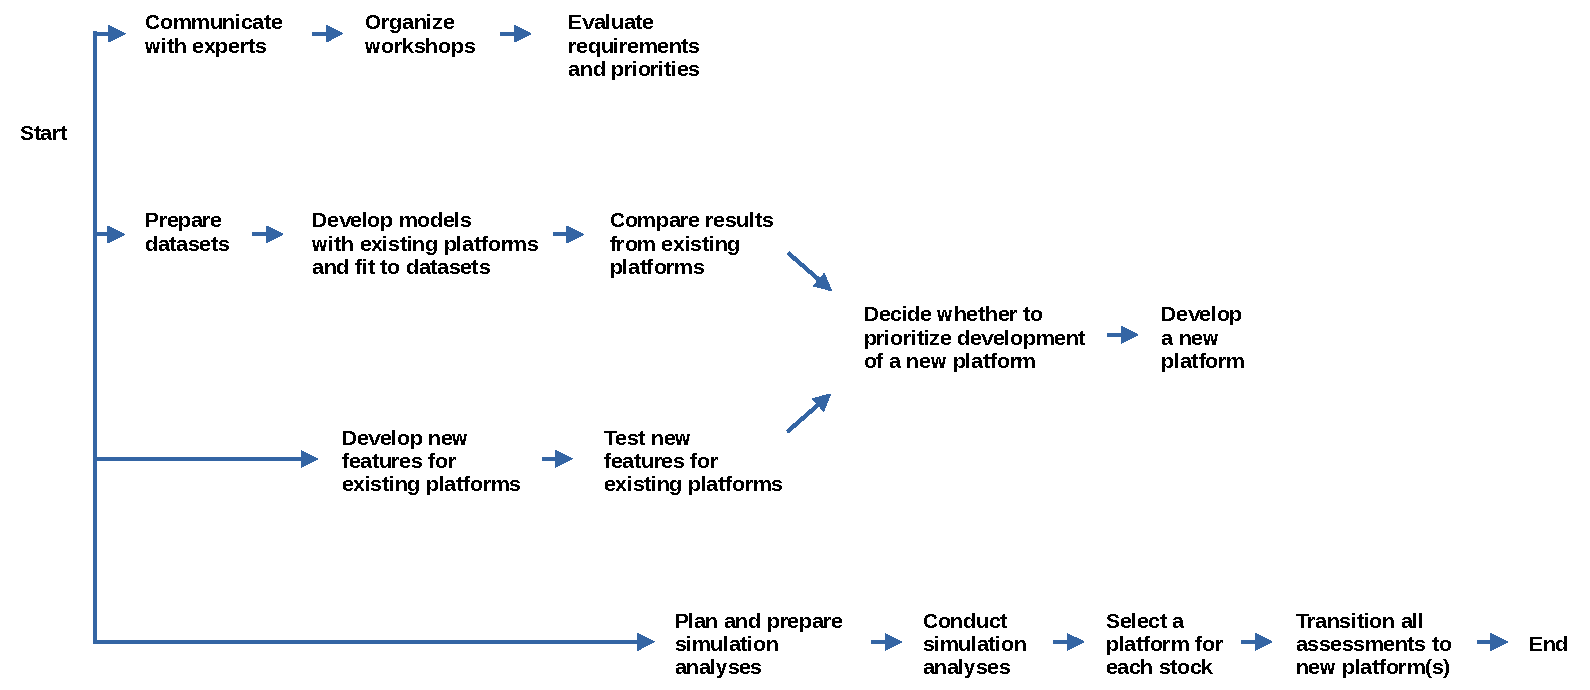
\includegraphics[width=\textwidth]{tasks_no_margin}
  \vspace{-1ex}
  \caption{Overview of tasks related to the next generation of tuna stock
    assessment software. Project~123 will focus on the first line of scoping
    tasks (communicate, organize, evaluate) and prepare the ground for
    subsequent lines of tasks (the main project), which will require additional
    funding and resources.}
\end{figure}

\section{Introduction}

\subsection{The need to migrate to new software}

Following the retirement of the lead developer of MULTIFAN-CL (MFCL), Dave
Fournier, future advances to the MFCL software are not expected to be as
mathematically innovative as they were in the past. While this does not render
MFCL obsolete in the medium-term, it flags the need to plan and identify whether
alternative existing software exists, or new software must be developed in the
longer-term, to continue to support the specificities and future requirements of
WCPFC tuna stock assessments.

While MFCL (Fournier et al. 1998) continues to be improved to service the WCPFC
tuna assessment needs over at least the next 5+ years, it is important to start
on a phased approach to its replacement. An initial scoping phase is required to
assess what features and capabilities will be important in future assessment
software for tunas. This scoping phase will benefit from input from stock
assessment scientists across global tuna RFMOs. Once this scoping phase is
conducted, consideration of available software packages in relation to the
desired features and capabilities can be conducted. This may identify suitable
existing software that has potential to provide the desired features and/or has
potential to be developed further. Alternatively, it may indicate whether
embarking on development of a new software package is recommended.

There has also been discussion around the need to explore, through
modeling/simulation exercises, the benefits of applying alternative assessment
structures (i.e., length-age structured versus the traditional length-based
age-structured approach of MFCL and Stock Synthesis) before embarking on major
software developments or changing methodology. Similar can be said about
exploring benefits of state-space models and their use of random variables.
Simulation exercises to explore the benefits or drawbacks of alternative model
structures or approaches will also require collaboration across tuna RFMOs and
experienced practitioners using the alternative approaches and/or software.

An important outcome of this work would be to ultimately have a software package
that has the desired functionality for tuna assessments, not only for WCPFC, but
globally, thus creating a user community and ongoing development support
capacity, so as to avoid the current situation we are facing with MFCL. Wider
collaboration in this venture is essential to achieving this and is expected to
be encouraged through this project.

\subsection{Project outline}

The project is divided into stages, as follows:

Year 2024

\begin{enumerate}
  \item Review and identify a list of necessary and desired features for
  software to conduct tuna stock assessments.
  \item Identify existing software platforms that have some or all these
  features or can be extended to add such features.
  \item Reach out to and initiate collaboration with developers who are already
  exploring extensions to current age-structured catch-at-age and state-space
  models that would allow those models to fit to length data.
  \item Conduct two workshops with selected experts from other tuna RFMOs and or
  with relevant expertise. The first workshop can be remote (prior to SC20) and
  the second one potentially in person (post SC20). The main goal will be to
  plan and document collaborative simulation studies to evaluate the performance
  of candidate software platforms for tuna stock assessments.
\end{enumerate}

Years 2025 and 2026 (subject to SC advice and funding approvals by WCPFC)

\begin{enumerate}\setcounter{enumi}{4}
  \item Conduct the simulation studies outlined in stage 4, in collaboration
  with experts that are supported by other agencies/RFMOs.
  \item Based on the results from simulation studies, determine which, if any,
  software platforms can be considered viable candidate platforms for WCPFC tuna
  assessments.
  \item If a viable candidate platform has been identified, provide a plan to
  transition assessments to this software. Evaluate which transitioned
  assessments could replace old MFCL assessments and build the transition into
  the WCPFC assessment schedule.
  \item If no viable candidate platform is identified, further extensions to
  existing platforms may be required, or the development of a new assessment
  software platform. The design process for a new platform would require
  additional development workshops and involvement of software developers
  (additional funds likely required) and could include identification of MFCL
  features and algorithms that can be borrowed and ported across to a new
  framework.
\end{enumerate}

\subsection{Existing software}

The CAPAM 2019 Workshop on Next Generation Assessment Models (Punt et al. 2020)
provided an overview and discussion of existing software, as well as
recommendations for further software development.

For the purposes of tuna assessments, the most relevant existing software (other
than MFCL) includes:

\begin{itemize}
  \item \textbf{Stock Synthesis} is used in tuna assessments by the IATTC, IOTC,
  and ICCAT. Migrating SPC assessments to Stock Synthesis would lose some of the
  features provided by MFCL and this would be transitioning to another platform
  that is expected to phased out in the \mbox{not-too-distant} future. On the
  other hand, increasing the use of Stock Synthesis at SPC would facilitate
  collaboration between the tRFMOs, including development of future models. It
  would also shorten the training time for new SPC stock assessors and make
  their skills and experience more transferable to subsequent workplaces. Stock
  Synthesis has a large user community that is relevant for peer reviews and
  discussing technical decisions. It also comes with an exceptionally complete
  suite of tools useful for diagnostics, as well as automated plots and tables
  for assessment reports. There is interest from SPC and the Stock Synthesis
  maintainers to explore the possibility of enhancing the tag module, see
  \autoref{sec:ongoing-upcoming-development}.
  \item \textbf{sbt} is used in the assessment of southern bluefin tuna by
  CCSBT. This package, implemented in TMB, stands out as the primary stock
  assessment software that is built around close-kin mark-recapture (CKMR) which
  is a new and important data type in upcoming SPC tuna assessments. The
  \textsf{sbt} R package is designed for a single-region assessment and would
  require some additional development to be used for a multiregion assessment.
  There is interest from SPC and the \textsf{sbt} maintainers to explore the
  possibility of adding multiregion functionality to the software.
  \item \textbf{Gadget3} is the latest version of Gadget stock assessment
  platform, implemented in TMB. Porting the software to TMB has resulted in a
  significant performance gain in terms of computational time. Gadget has a wide
  range of features relevant for tuna assessments and there is interest from SPC
  and the Gadget maintainers to test its use for a tuna assessment.
  \item \textbf{Casal2} is the latest version of the Casal stock assessment
  platform, rewritten with an improved design and user interface. Casal has a
  wide range of features relevant for tuna assessments and there is interest
  from SPC and the Casal maintainers to test its use for a tuna assessment.
  \item \textbf{Stock Synthesis + CKMR} is an experimental add-on to Stock
  Synthesis (A.E. Punt, pers. comm), adding CKMR as a data type in Stock
  Synthesis. This was successful as a proof of concept but is not very likely to
  be added to the core software.
\end{itemize}

\subsection{Ongoing and upcoming software development}
\label{sec:ongoing-upcoming-development}

Some ongoing software development projects are of particular interest in the
context of the next SPC tuna assessment models:

\begin{itemize}
  \item \textbf{ALSCL + Fleets} is a recent and simple model that has two
  important features: state-space formulation and age-length structure. It is
  implemented in TMB, but the software currently fits only to survey data and
  does not include commercial catches or fleets. There is interest from SPC and
  the ALSCL maintainers to explore the possibility of adding commercial catches
  and fleets as software features.
  \item \textbf{Stock Synthesis + Enhanced Tags} is a proposed software
  development of an enhanced tag module for Stock Synthesis. The current
  implementation of fitting to tagging data is somewhat limited, e.g., requiring
  the user to enter the age at release, which is not available in tuna
  assessments. The idea is to borrow some of the functionality and features from
  the tag module in MFCL, which has a long record of using tagging data as a
  primary data type in tuna assessments. There is interest from SPC and NOAA
  scientists to explore the possibility of contributing an enhanced tag module
  to be incorporated into the core Stock Synthesis software.
  \item \textbf{WHAM + Length} is a recent software development (Correa et al.
  2023) extending the state-space stock assessment software WHAM (Stock and
  Miller 2021) to fit to length data. There is interest from SPC and AZTI
  scientists to experiment with fitting the WHAM + Length model to an SPC tuna
  assessment dataset.
  \item \textbf{SAM + Length} is an early exploration of extending the
  state-space stock assessment software SAM (Nielsen and Berg 2014) to fit to
  length data. There is interest from SPC and DTU/ICES scientists to continue
  this exploration.
\end{itemize}

\section{Possible tasks for SPC to prioritize}

\subsection{Migrate assessments to existing software}

\begin{enumerate}
  \item Move the swordfish assessment to Stock Synthesis. The swordfish
  assessment is relatively simple compared to other SPC assessments and would be
  a good candidate to be the first to migrate from MFCL. The 2025 swordfish
  assessment could be developed in a stepwise progression: previous MFCL
  diagnostic $\Rightarrow$ catch-conditioned MFCL $\Rightarrow$ Stock Synthesis.
  \item Move the striped marlin assessment to Stock Synthesis. The striped
  marlin assessment is also relatively simple and would be a good candidate to
  migrate from MFCL. Currently, the next striped marlin assessment is planned in
  2029, but an update assessment could be conducted in 2025, 2026, or 2027,
  depending on the resources committed to this task. The update assessment could
  be put forward as the basis of scientific advice or as a technical milestone.
\end{enumerate}

\subsection{Exploratory analyses using existing software}

\begin{enumerate}\setcounter{enumi}{2}
  \item Conduct exploratory analyses to fit Casal/Gadget/Stock Synthesis to
  albacore tuna. The albacore assessment is simpler than the other tuna species
  and therefore a candidate to be the first tuna stock to migrate from MFCL.
  \item Conduct exploratory analyses to fit Casal/Gadget/Stock Synthesis to the
  original five-region yellowfin tuna dataset. The yellowfin assessment is a
  good candidate to test the capabilities of these software platforms for tuna
  assessments involving multiple regions, tags, and a large number of fisheries.
  The yellowfin tuna assessment is similar to bigeye tuna but runs slightly
  faster, thanks to the simpler \mbox{five-region} structure that was adopted in
  the 2023 assessment.
  \item Conduct exploratory analyses to fit models using a variety of existing
  software to a simplified single-region yellowfin tuna dataset. Models of
  interest include ALSCL, Casal, Gadget, MFCL, sbt, Stock Synthesis, and
  WHAM+Length.
\end{enumerate}

\subsection{Software development}

\subsubsection{Extend existing software}

The benefits and rationale of the following software extensions are described in
\autoref{sec:ongoing-upcoming-development}. The prioritization and duration of
these tasks may depend on the initial findings of these and other tasks,
available resources, and the availability of external scientists involved.

\begin{enumerate}\setcounter{enumi}{5}
  \item ALSCL+Fleets. Scientists involved could include Fan Zhang (Shanghai
  Ocean University) and Nick Davies (SPC).
  \item Stock Synthesis+Enhanced Tags. Scientists involved could include
  Nicholas Ducharme-Barth (NOAA), Matthew Vincent (NOAA), and Arni Magnusson
  (SPC).
  \item WHAM+Length. Scientists involved could include Giancarlo Correa (AZTI)
  and Arni Magnusson (SPC).
  \item SAM+Length. Scientists involved could include Anders Nielsen (DTU),
  Colin Millar (ICES), and Arni Magnusson (SPC).
\end{enumerate}

\subsubsection{Design and develop new software for tuna assessments}

\begin{enumerate}\setcounter{enumi}{9}
  \item Initial explorations using RTMB, starting with simple model development
  and gradually adding complexity and tests. Scientists involved could include
  Nick Davies (SPC) and Arni Magnusson (SPC).
\end{enumerate}

\section{Timeline}

\subsection{International expert meeting 2024}

\subsubsection{Objectives}

The meeting objectives were:

\begin{enumerate}
  \item Communicate SPC scoping project and upcoming explorations, decisions,
  and development.
  \item Discuss succession plans for MULTIFAN-CL as well as Stock Synthesis.
  \item Seek advice from the scientific community.
  \item Seek collaboration with tuna RFMOs and various research labs.
\end{enumerate}

\subsubsection{Format}

Two online meetings were held on 13 May and 18 June 2024, inviting stock
assessment and software development experts from around the world. The two
sessions had the same format and agenda, but one was centered on European time
zones and the other on North American time zones. Around 40 participants
represented the tuna RFMOs (CCSBT, IATTC, ICCAT, IOTC, WCPFC), stock assessment
software projects (ALSCL, CASAL, FIMS, Gadget, MFCL, SAM, sbt, Stock Synthesis,
WHAM), and maintainers of relevant programming languages (ADMB, RTMB, TMB).

The meeting agenda covered the following discussion topics:

\begin{itemize}
  \item Platforms currently used in tuna stock assessments\\[-4ex]
  \item Common challenges for all tuna RFMOs, longevity of Stock Synthesis and
  MULTIFAN-CL, succession plans\\[-4ex]
  \item SPC challenges and project plan\\[-4ex]
  \item Features of current and future platforms\\[-4ex]
  \item Discussion on platform features most relevant for tuna\\[-4ex]
  \item State-space models and latest developments\\[-4ex]
  \item What do you think is the best way forward for SPC?\\[-4ex]
  \item Summary of discussions, next steps, collaboration
\end{itemize}

\subsubsection{Outcomes}

There was a consensus among the experts that the goal should be to design and
develop a model specific for tuna assessments, rather than a general model for
global usage and all species. The advice was to start with a lean design and get
a simple model up and running before adding all the features required for an
assessment. In general, the cost of adding features is much greater than the
implementation cost, as each layer complexity makes long-term maintenance and
future modifications of the software more difficult and costly.

RTMB (Kristensen 2024) is a new alternative interface for developing TMB
(Kristensen et al. 2017) models. RTMB provides a leaner development paradigm
than TMB. The recommendation from the TMB/RTMB development team, articulated at
the expert meeting, was to develop the next tuna stock assessment model in RTMB
rather than TMB. Another recommendation from the TMB/RTMB development team,
given the streamlined nature of RTMB model implementation is for SPC to consider
writing specific models for each species, rather than a general platform for all
species and tRFMOs. A specific RTMB model requires a very small codebase that is
easy to maintain and modify. Parts of code can still be reused between species,
either as code blocks or functions.

State-space models are a statistically and computationally efficient way to
allow time-varying processes in stock assessment models, such as time-varying
selectivity. Other statistical approaches exist, but the successful track record
of using state-space models in production assessments, e.g., across a variety of
Atlantic groundfish stocks, indicates that state-space formulation can be
recommended for new model development.

Age-length structure is explicitly tracked in Gadget models, accounting for the
fact that fast-growing individuals are caught by the fishery and the
slow-growing individuals in the cohort remain in the population. Casal and Stock
Synthesis have optional model features with a similar aim. This leads to an
improved level of realism, and simulations using a very basic model ALSCL (Zhang
and Cadigan 2022) indicate improved estimation accuracy. It is worth noting that
the ALSCL simulation study involved a single-area model with survey data and no
commercial catch data or fleets, which is quite far from the model complexity of
tuna assessments. An important drawback is that tracking the population
structure in terms of age and length, instead of age only, comes at a
considerable computational cost. The SPC tuna assessment models that are
currently run in MFCL are already very computationally heavy, with models
requiring to run overnight before results are available. The recommendation is
to explore the feature of incorporating full age-length structure in the next
tuna assessment models, considering estimation performance and the difference in
the resulting management advice, as well as computational time, required
software development, and maintenance cost.

The discussion at the international expert meeting covered several other topics,
but the above recommendations are particularly relevant for initial explorations
and development. In addition to the discussion and recommendations, an important
outcome of the international expert meeting was to establish collaboration with
various research labs related to the development of new tuna assessment models.
See next section.

\subsection{Workshop activities in 2024--2026}

\subsection{Launching the main project}

\section{Required resources}

\subsection{Collaboration with other tRFMOs}

\subsection{SPC staff positions, consultants}

\section{References}

\sloppy\setlength\hyphenpenalty{1000}

\begin{description}\setlength\itemsep{0ex}
  \item Correa, G.M., C.C. Monnahan, J.Y. Sullivan, J.T. Thorson, and A.E. Punt.
  2023. Modelling time-varying growth in state-space stock assessments. ICES J.
  Mar. Sci.80:2036--2049.
  \item Fournier, D.A., J. Hampton, and J.R. Sibert. 1998. MULTIFAN-CL: A
  length-based, age-structured model for fisheries stock assessment, with
  application to South Pacific albacore, \textit{Thunnus alalunga}. Can. J.
  Fish. Aquat. Sci. 55:2105--2116.
  \item Kristensen, K. 2024. RTMB: R bindings for TMB. R package version 1.5.\\
  https://cran.r-project.org/package=RTMB.
  \item Kristensen, K. A. Nielsen, C.W. Berg, H. Skaug, and B.M. Bell. 2016.
  TMB: Automatic differentiation and Laplace approximation. J. Stat. Softw.
  70(5):1--21.
  \item Nielsen, A. and C.W. Berg. 2014. Estimation of time-varying selectivity
  in stock assessments using state-space models. Fish. Res. 158:96--101.
  \item Punt, A.E., A. Dunn, B.Þ. Elvarsson, J. Hampton, S.D. Hoyle, M.N.
  Maunder, R.D. Methot, and A. Nielsen. 2020. Essential features of the
  next-generation integrated fisheries stock assessment package: A perspective.
  Fish. Res. 229:105617.
  \item Stock, B.C. and T.J. Miller. 2021. The Woods Hole Assessment Model
  (WHAM): A general state-space assessment framework that incorporates time- and
  age-varying processes via random effects and links to environmental
  covariates. Fish. Res. 240:105967.
  \item Zhang, F. and N.G. Cadigan. 2022. An age-and length-structured
  statistical catch-at-length model for hard-to-age fisheries stocks. Fish and
  Fish. 23:1121--1135.
\end{description}

\end{document}
